\chapter{Design and Implementation}

This chapter provides details regarding the FMLearn application, implementation of the proposed concept, that is, Federated meta Learning and it's working mechanisms. Each component of the application is discussed in detail including the components what were considered and tested, but are not a part of the final experimentation. Explanation of each design decisions are also provided in detail so as it make it easier for the reader to understand how the application developed over-time and reached it's final state. The FMLearn application will attempt to solve the issue of redundant work put in by developers to find the best algorithm and it's hyper-parameters over and over again for a previously solved / optimised dataset and possibility suggesting algorithms for a previously unseen dataset as well. If this is achieved, the users of this application and the community in general will be greatly benefited by saving time spent waiting for program to complete, electricity consumed on the running the machines and cooling them, the computational power expended over a repetitive task and money spent in all of the above, to find the best algorithm and it's hyper-parameter.

The design and implementation choices led to the development of a working prototype of the concept Federated Meta-Learning and the application FMLearn. The server was developed in Python and exposed the capabilities of the application as publicly available API's which uses a the standard JSON format for sending and receiving data / information. The concept of Federated Meta-Learning discussed in \ref{federated-meta-learning}

\section{Requirements}
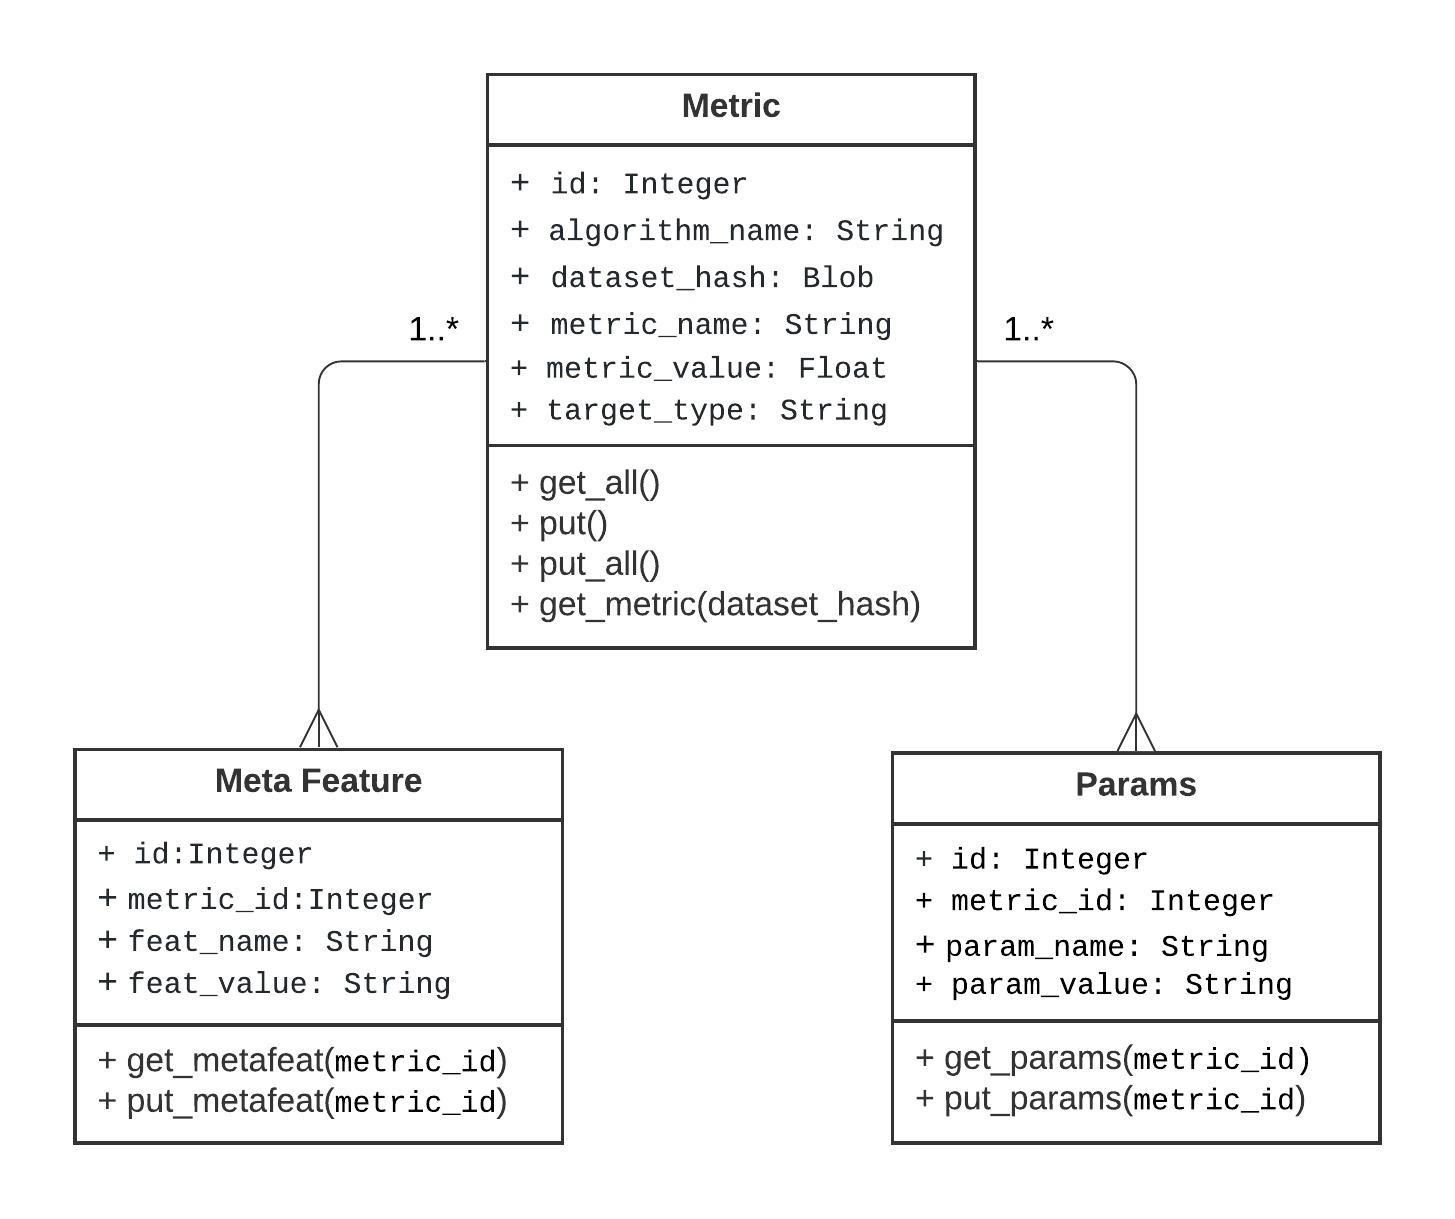
\includegraphics{images/Class Diagram.jpeg}
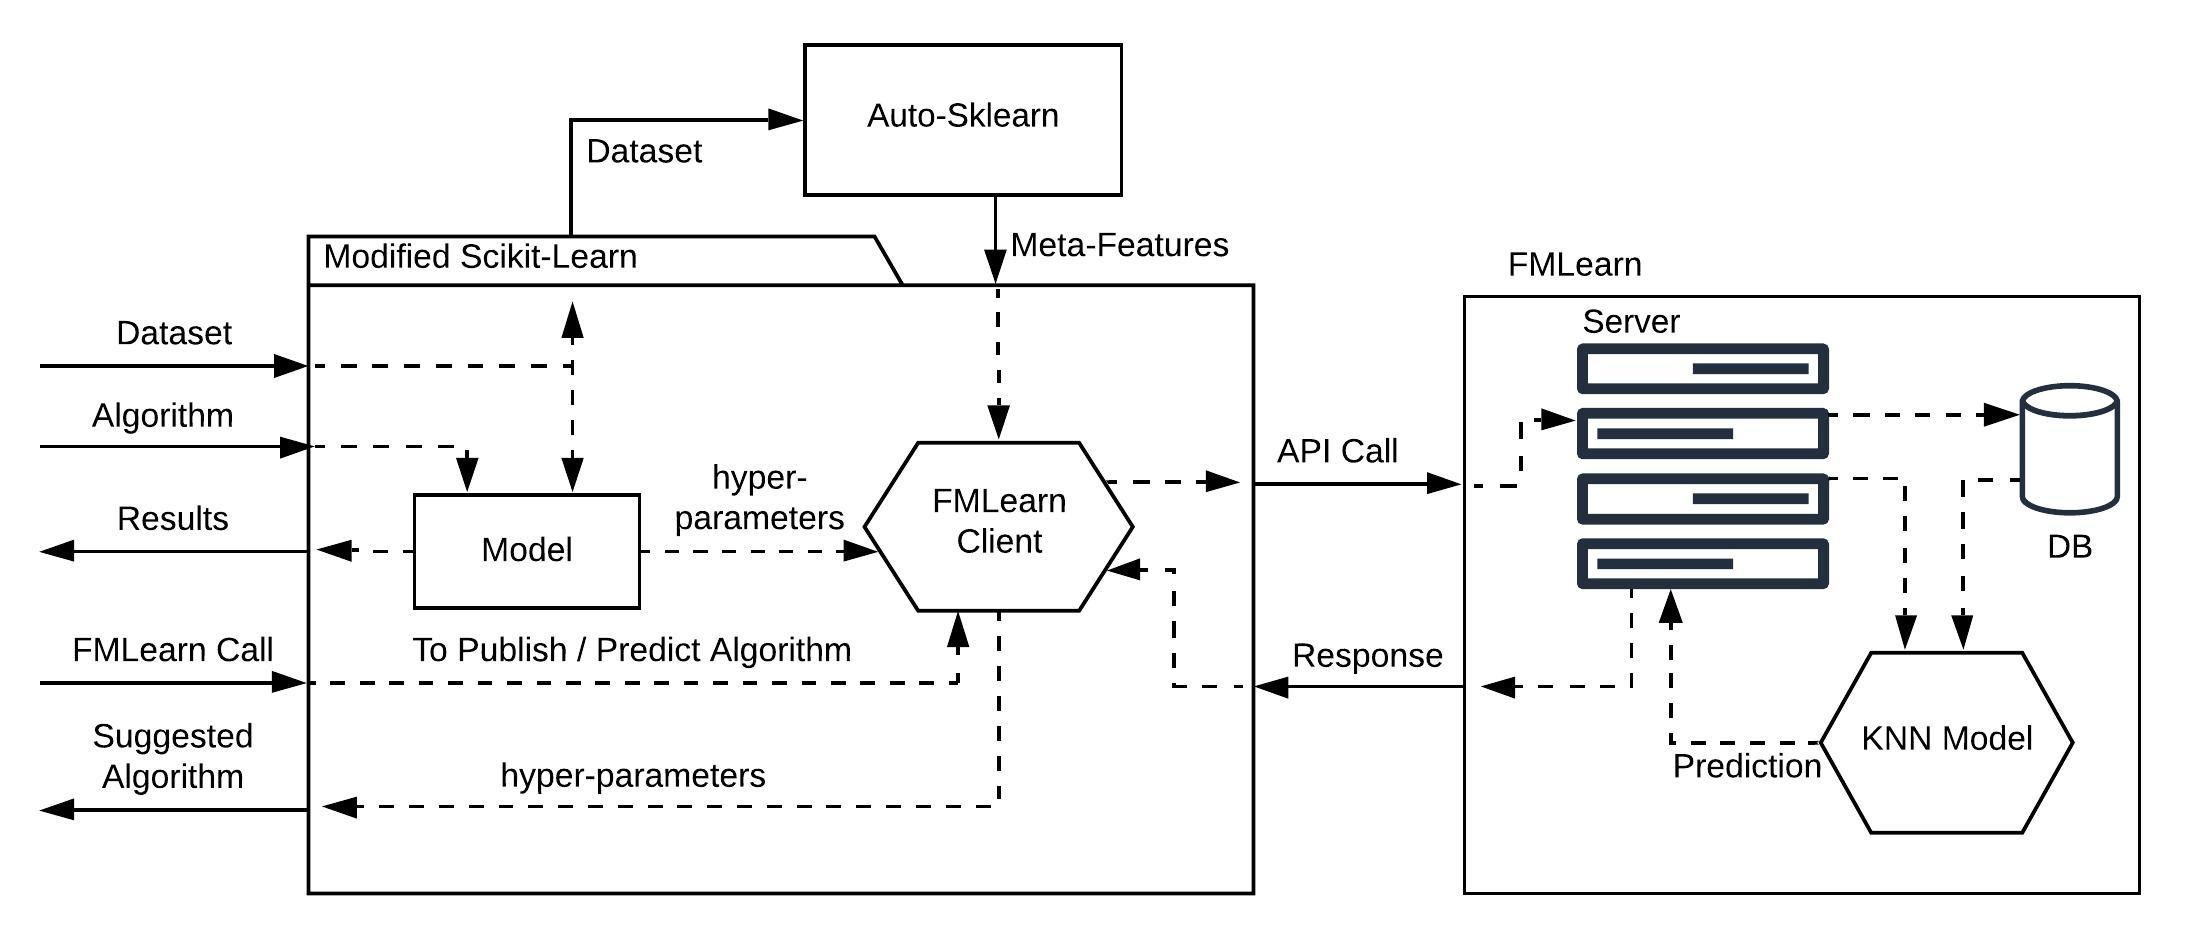
\includegraphics{images/FML Architecture Diagram.jpeg}
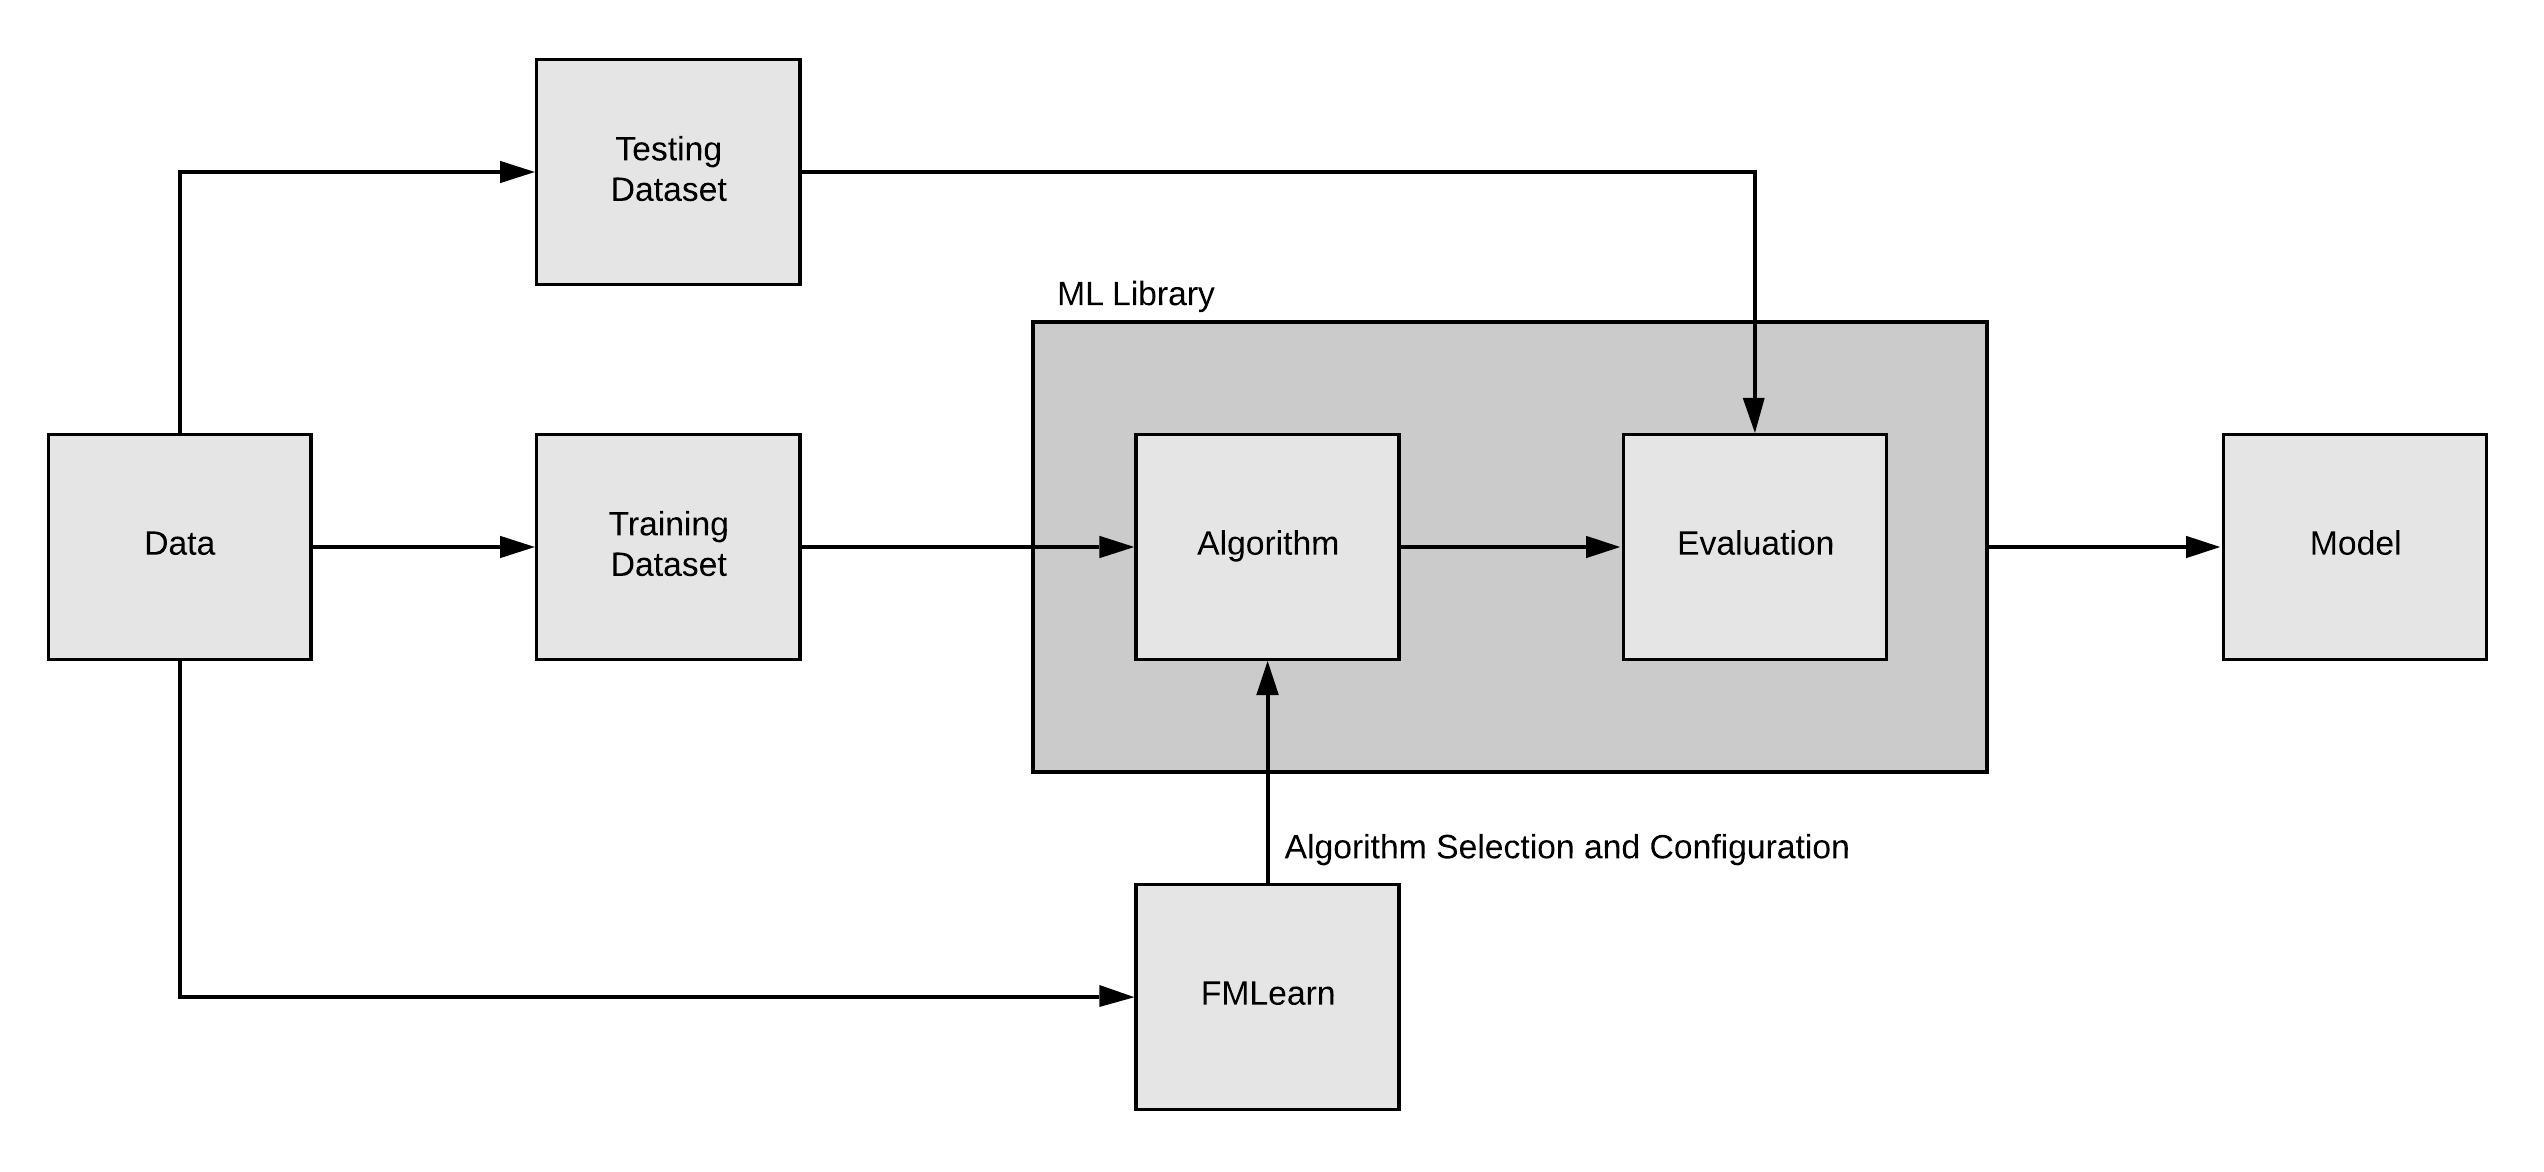
\includegraphics{images/FML Workflow.jpeg}
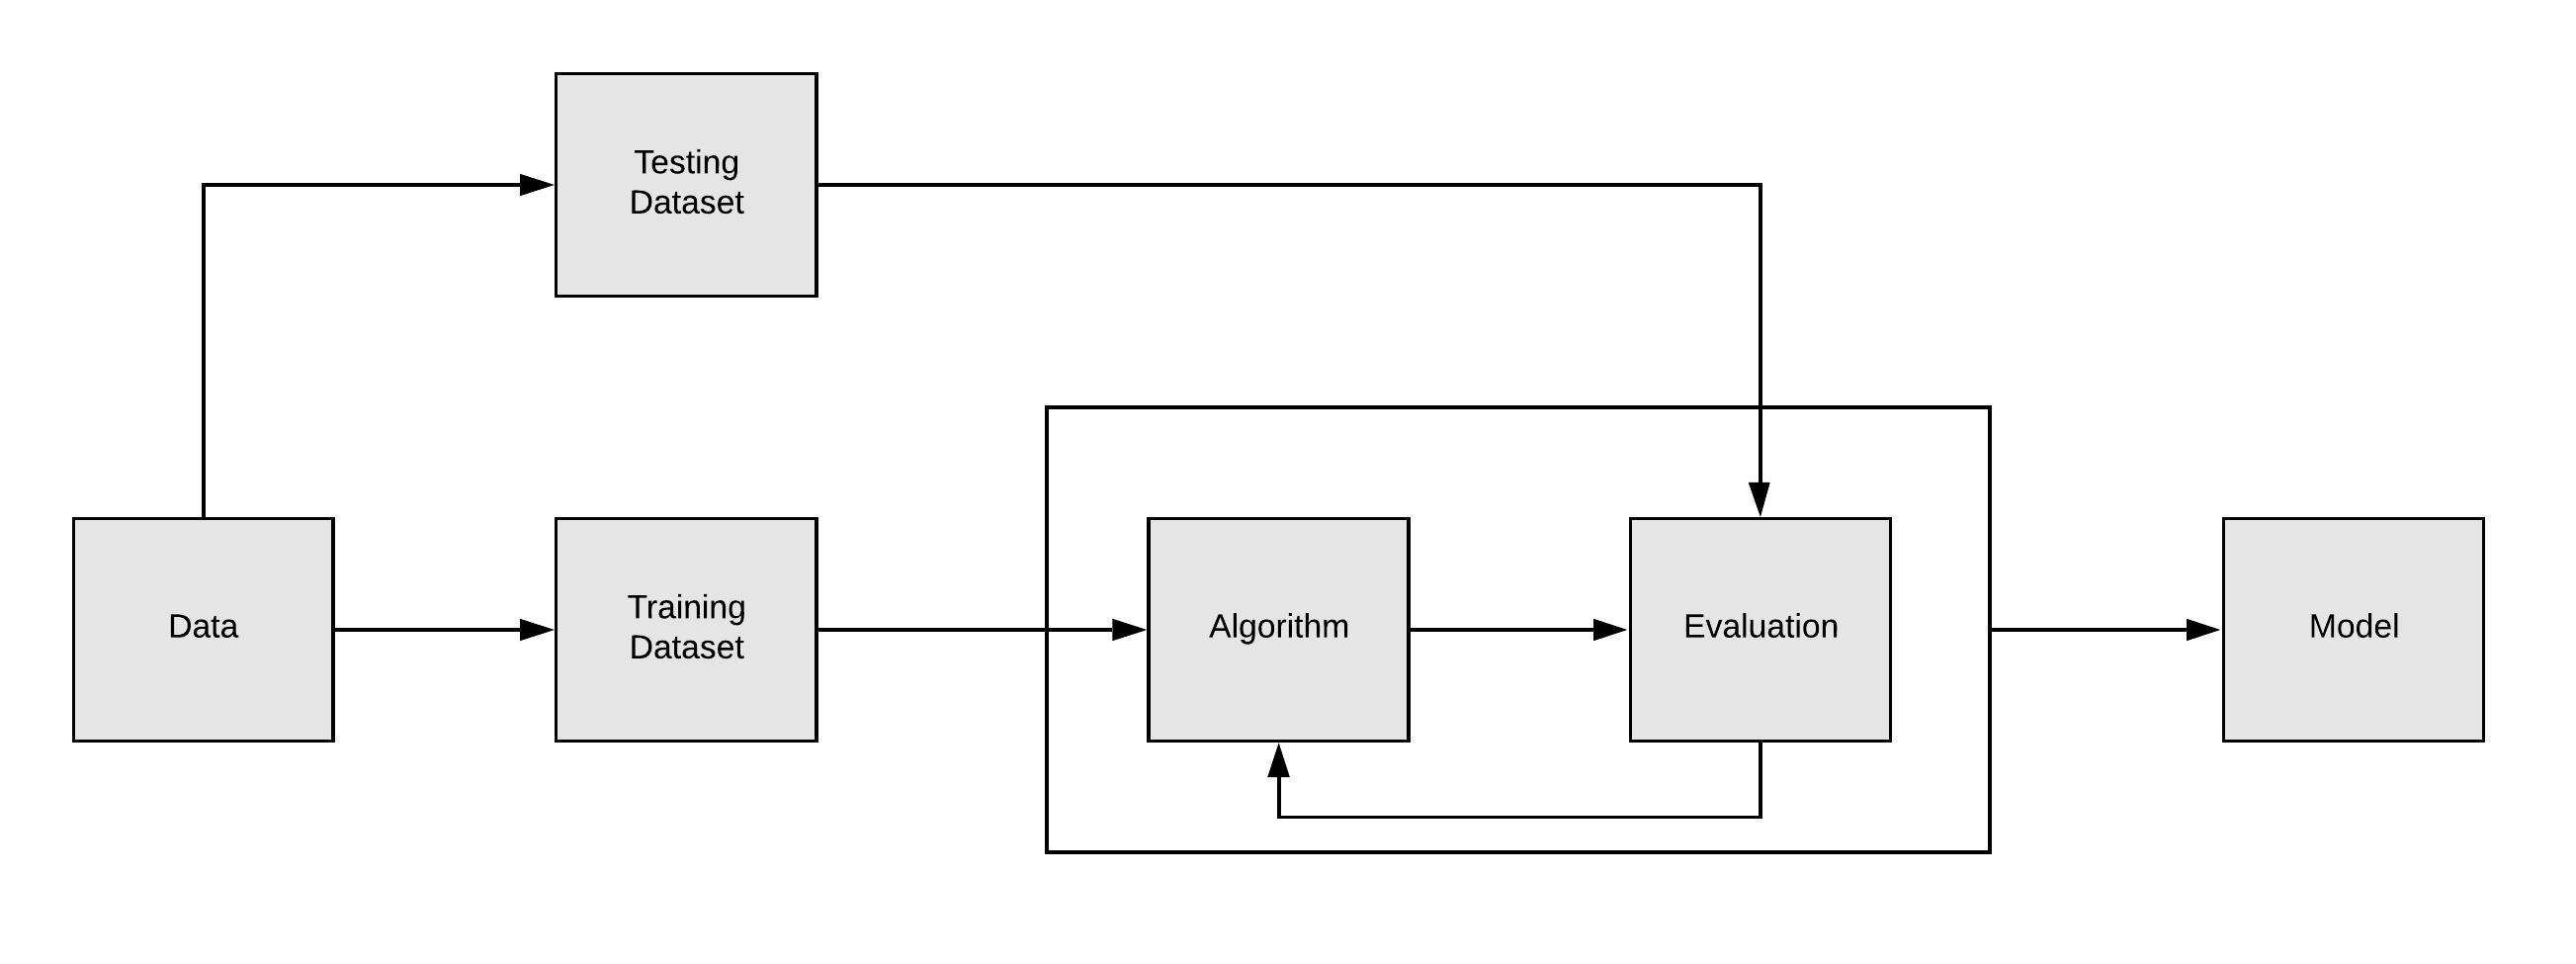
\includegraphics{images/ML Workflow.jpeg}
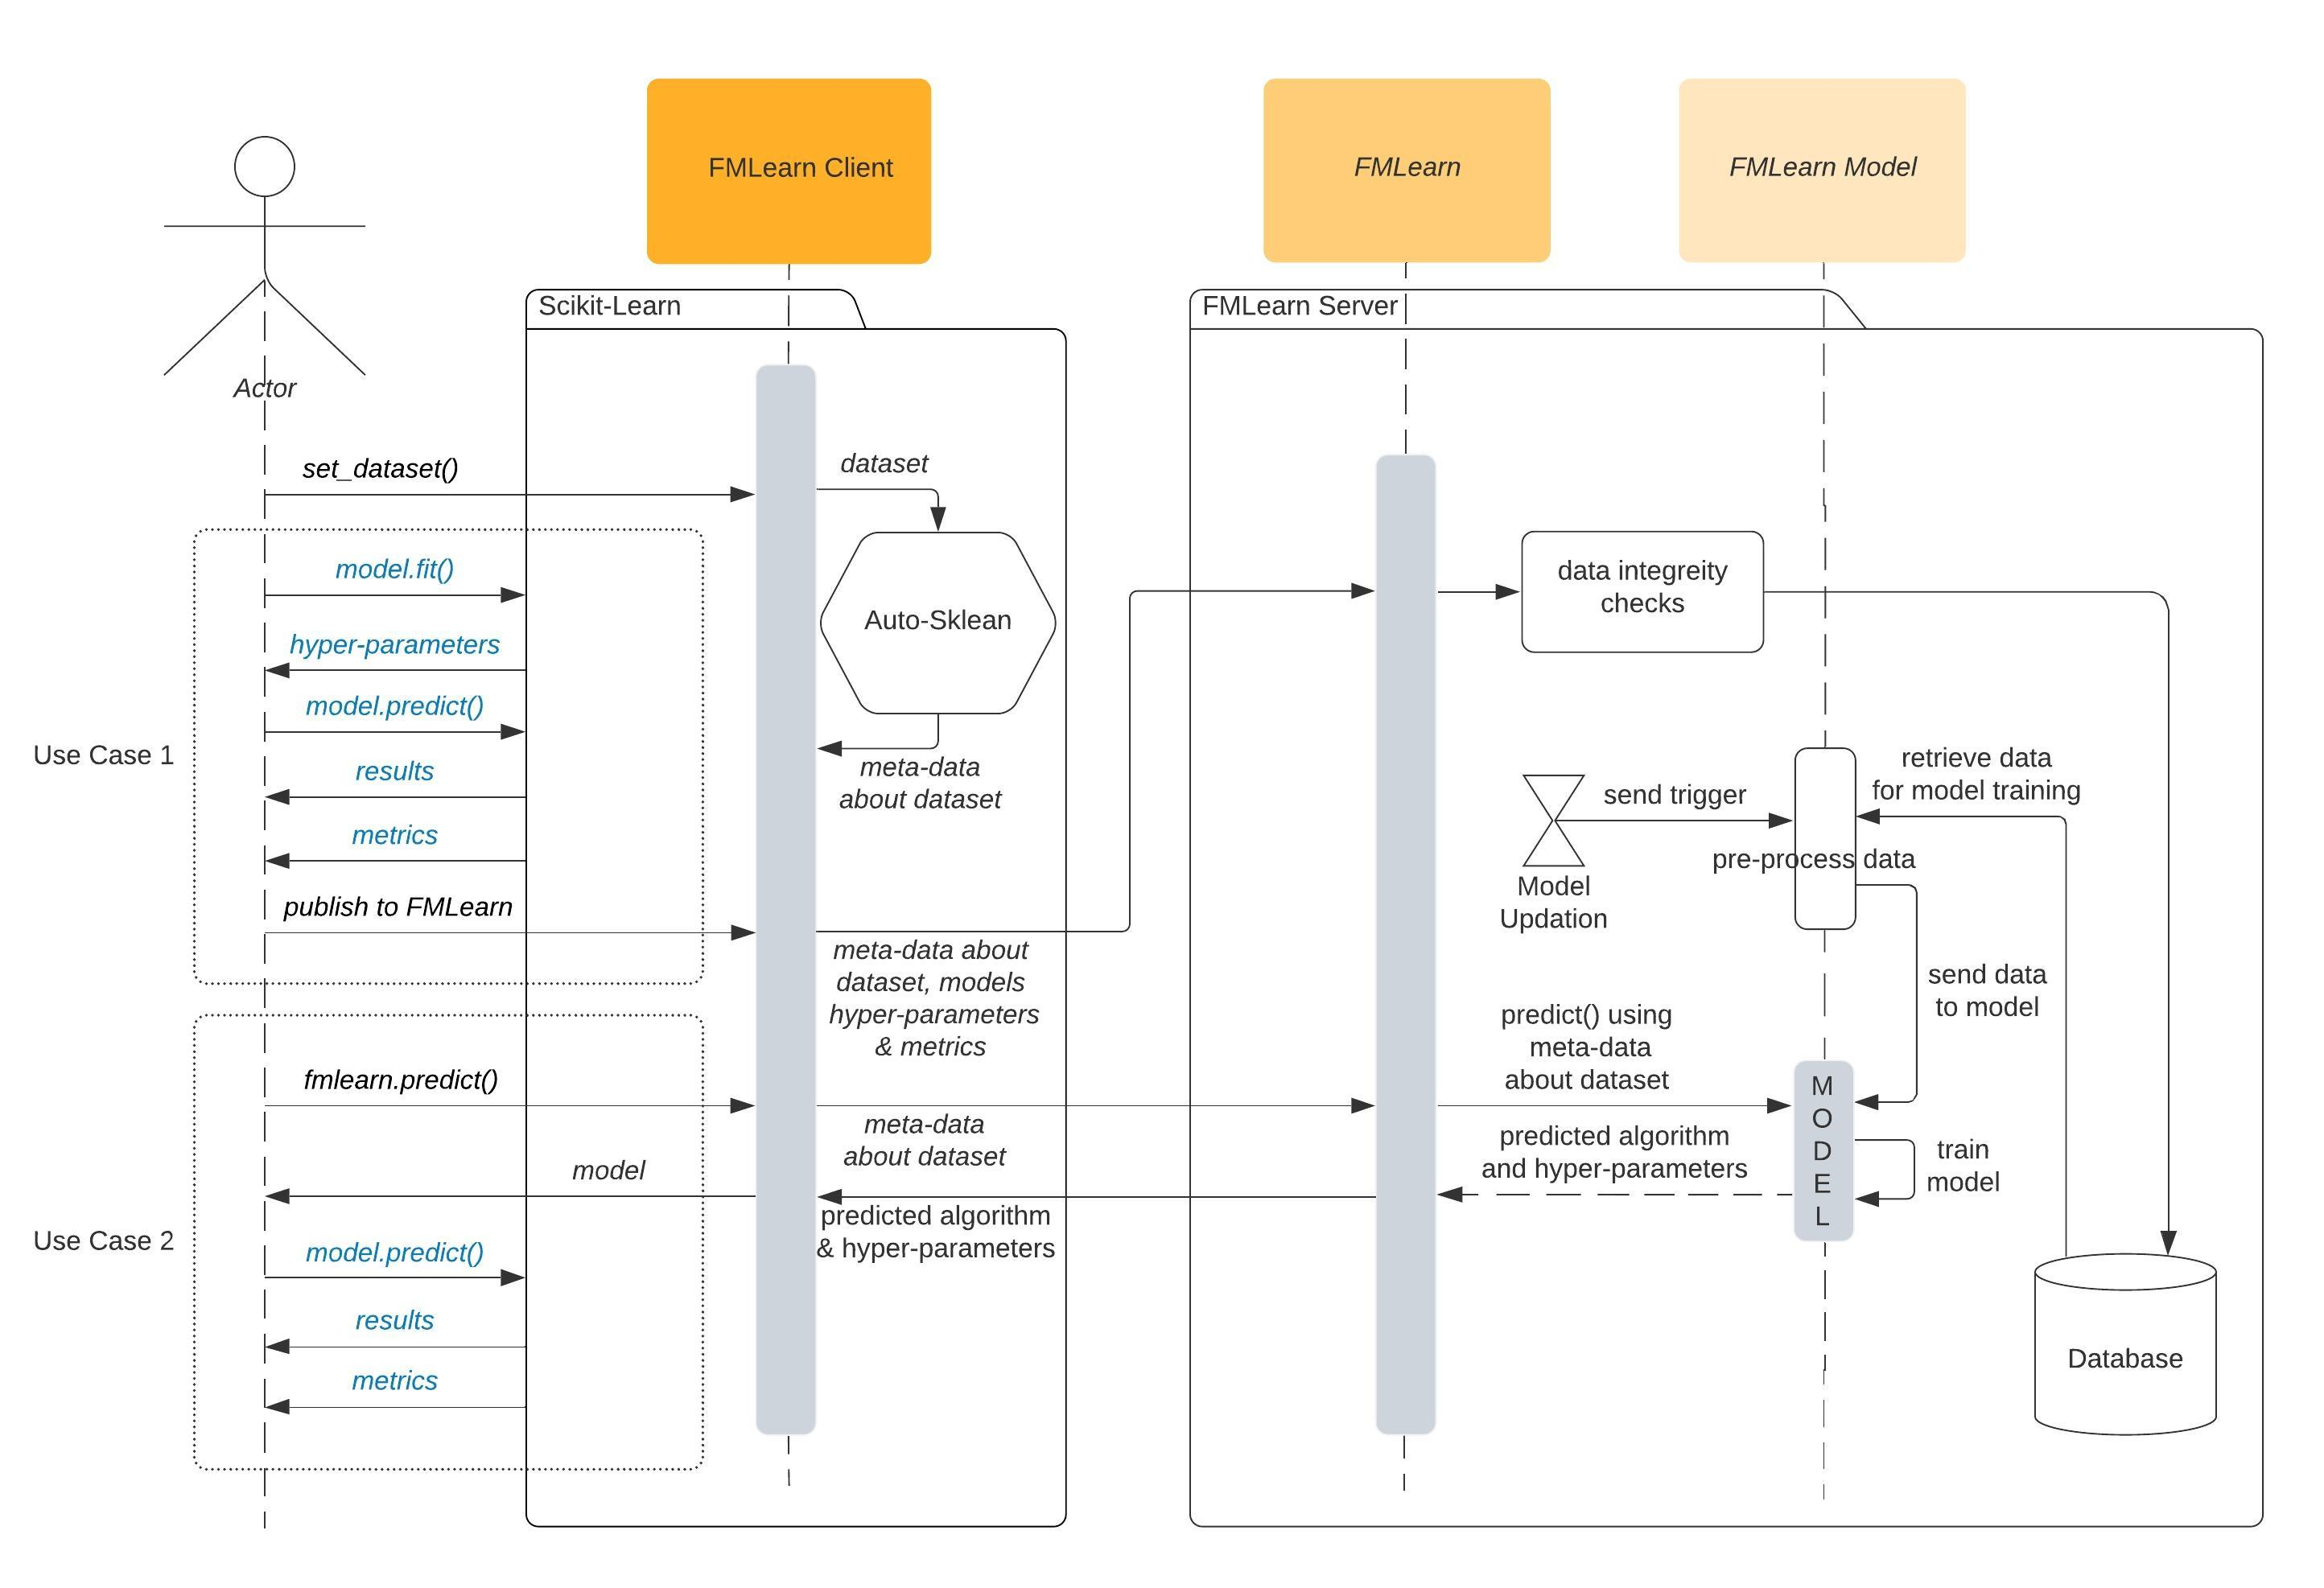
\includegraphics{images/Sequence Diagram.jpeg}

\section{High-Level Overview}

\section{Federated Meta-Learning}
\label{federated-meta-learning}

\section{SciKit-Learn}
\label{scikit-learn}

\subsection{Auto-Sklearn Meta Features}
\label{auto-sklearn}

\subsection{Knowledge Base building}
\label{knowledge-base}

\section{FMLearn}
\label{fmlearn}

\subsection{Architecture Design}
\label{architecture}

\subsection{Design Decisions}
\label{design-decisioins}

\subsection{ML Algorithm}
%%\subsubsection{Why this algo}
%%\subsubsection{results of others}
%%\subsubsection{comparison between other algos}
\subsection{Workflow}

\section{Security and Privacy Concerns}
FMLearn is a client-server architecture-based [2] application which provides public API’s for it's users, and it brings its own security and privacy concerns. The different aspects of security and privacy issues that are to be considered with respect to FMLearn are - but not limited to:

\begin{enumerate}
    \item A client-server architecture.
    \item Publicly available API server [3] (which could be broken down)
\end{enumerate}

\subsection{Security Concerns}

FMLearn was built using Python Flask, and uses PostgreSQL, which acts as the public API server which exposes various API to users to use the application and is currently hosted on Heroku .

One of the most important security concerns with the current implementation of FMLearn is that the users have unlimited access to APIs (Flash Crowd Problem) [4], this could have severe consequences. A denial of service is possible, and extraction of all information of few of the major effects. This could be resolved using various rate-limiting strategies:

\begin{itemize} 
    \item Limiting per connection property (IP address)
    \item Limiting per user (account / access token / API key)
    \item Limiting per application property (user account / resource type)
    \item Limiting based on context (region / type of app)
\end{itemize}

Once these rate-limiting features have been introduced if someone tried to repeatedly access the API, they would get the following error.

\quad\quad\quad\quad\quad\quad\quad\quad\quad\quad\quad\quad\quad
\texttt{HTTP/1.1 429 Too Many Requests}\\
\quad\quad\quad\quad\quad\quad\quad\quad\quad\quad\quad\quad\quad
\texttt{Retry-After: 3600}


Rate limiting prevents malicious code from abusing legitimate / illegitimate access to the API.

One of the basic and yet most powerful technique which helps prevent a lot of security issues is Input validation [5]. Input validation should act as the first line of defense in case of a malicious attack. It is also useful to reject malicious data which helps prevent DoS attacks by rejecting unreasonably large inputs and against injection attacks by rejecting crafted payloads. Some of the possible Input validation techniques which could be easily enforced in my case are:

\begin{itemize}
    \item Enforcing sensible length limits on inputs.\\
    (i.e., 2MB of user’s hashed dataset is not allowed)
    \item Enforcing strict content types on provided data inputs.\\
    (i.e., an API expecting JSON data should not accept anything else.
    \item Enforcing strict data type checking on inputs.\\
    (i.e., Numbers should be numbers, and SQL code as input results in an error)
\end{itemize}

Even though input validation is a decent first line of defense, it will fail if used as the only line of defense because when the application evolves and brings in complex input types it will not prevent attacks as it will be complex to determine the validity of complex data at input time. Moreover, complex validation procedures usually suffer from bypass attacks, and making validations might break functionality. [6]

\subsection{Data Protection}
Another possible issues specific to FMLearn is the storage of hash for the complete dataset in the proposed prototype, the dataset is hashed using sha256 though this is very secure it has its own set of vulnerabilities [7] that need to be taken into consideration, for now we can assume that sha256 is safe to use. But if it is broken there is a possibility that all the user data can become compromised. Even if the hash of the dataset is not broken, but if the meta-data about the model (like the model parameters) and dataset is available to the hacker, it is very much possible that a model could be reconstructed and the data of the user can be compromised.

Currently FMLearn is also vulnerable to Eavesdropping Attack, this is because the data sent from scikit-learn to FMLearn is not encrypted and is in plain-text, so various sniffing tools like Wireshark, Nmap, etc., can be used to monitor the network traffic and sniff the data transmitted between client and the server. To prevent such attacks, I can use a technique similar to twitter’s developer API access, where in the user is required to create an account with FMLearn and is required to use certain keys generated during account creation:

\quad\quad\quad\quad\quad\quad\quad\quad\quad\quad\quad\quad\quad\quad
\texttt{ACCESS\_TOKEN = ''\\}
\quad\quad\quad\quad\quad\quad\quad\quad\quad\quad\quad\quad\quad\quad
\texttt{ACCESS\_TOKEN\_SECRET = ''\\}
\quad\quad\quad\quad\quad\quad\quad\quad\quad\quad\quad\quad\quad\quad
\texttt{API\_KEY = ''\\}
\quad\quad\quad\quad\quad\quad\quad\quad\quad\quad\quad\quad\quad\quad
\texttt{API\_SECRET\_KEY = ''}

This introduces a 3-legged oauth authentication workflow similar to twitter’s developer API [8] access and these tokens can them be used to securely transfer data back and forth between the client and server, without worrying about eavesdropping attack. But then by introducing this we bring in new security vulnerabilities into the application which needs to be addressed separately in a larger scale. But for now sticking to just encrypting the information related to dataset let it be dataset hash or meta-data about the data, can be done as the first step in the necessary direction for this dissertation to proceed using public key encryption techniques. Doing just this helps protect the privacy of the user’s data from potential sniffers and maintains the integrity of the data over the network.

The scope of improvement in terms of security is huge in this project, it can be made secure enough for users to confidently use, but all this is just until things don’t go wrong.

\subsection{Social Concerns}
In the long run, social questions need consideration such as preventing manipulation (developers of algorithms may have an interest that their algorithms are "recommended") and free-rider problems (users benefiting from the system without sharing their data).

